\documentclass{article}
\usepackage[parfill]{parskip}
\usepackage{graphicx}
\usepackage{float}
\usepackage{placeins}
\usepackage[top=2 cm, bottom=2 cm, left=2 cm, right=2 cm]{geometry}
\usepackage{amsmath}

\usepackage[
    backend=biber,
    style=alphabetic,
    sorting=none
]{biblatex}
\addbibresource{bibliography.bib}

\title{Modeling project: DNA packaging in a virus}
\author{}
\date{}

\begin{document}

\maketitle

\begin{abstract}
\noindent
In order to infect a host cell, bacteriophage viruses must eject their genome, which is then replicated, followed by the synthesis of the proteins encoded in it. Once the concentration of the proteins is high enough, the construction of the viral capsids, which are rigid protein boxes, is initiated. The next step is the packaging of the viral DNA inside the capsids, which can then be injected into other host cells. The packaging of DNA in these viruses is thus an essential step in their life cycle. In this article, we describe a simple physical model explaining this packaging process for diversely shaped capsids. 
\end{abstract}


\section{Introduction}
The dynamics of the packing of double-stranded DNA in bacteriophages and other viruses using the same mechanism (ATP-dependent packaging of the DNA into a preformed capsid) has been investigated both experimentally and theoretically. There are two main types of theoretical models: thermodynamic quasi-static models which considers DNA as a polymer (see \cite{phillips2005}) and molecular dynamics models which simulate it as a series of beads connected by springs (see \cite{Petrov2008}). These two approaches lead to different predictions and there is still a debate about the nature of the dynamics and the forces involved in the mechanism.\cite{Berndsen2014} The physical model we present is of the former type. It assumes that DNA takes a single conformation inside the capsid and organizes itself as a spool. However, the first experimental measurement of the spatial organization of DNA inside the capsid during the packing process has only been observed in 2008 by Comoli and al. \cite{comoli2008}. They showed that contrarily to what was believed before (for instance in \cite{phillips2005, purohit2003}), DNA tends to organize itself in the spool structure very late in the packaging process. Indeed, until $78\%$ of the genome is packed, the DNA inside the capsid stays in a disordered phase. Thus, the dynamics of DNA packing inside viruses is still an active subject of research. 

%Que faire du tableau ??

\begin{table}[h]
    \centering
    \begin{tabular}{|| r | c | c | l ||}
        \hline \hline
        \textbf{Name of the variable} & \textbf{Symbol} & \textbf{Value} & \textbf{Source} \\
        \hline \hline
        Diameter of the capsid  & $R_{out}$   & $21\times 54~nm$ & Phage $\phi29$ \cite{tao1998}  \\
        Diameter of the DNA    & $ d_{dna}$  & $1~nm$           & \cite{phillips2005} \\
        Length of the DNA strand & $ L_{tot}$  & $5.5.10^{3}~nm$  & Phage $\phi29$ \cite{tao1998} \\
        Persistence length       & $ \xi_p $   & $50~nm$           & \cite{smith2001} \\
        Gyration radius          & $ R_{G} $     & $300~nm$         & phage $\phi29$ \cite{phillips2005} \\
        Motor force              & $ F_{mot}$  & $10~pN$          & \cite{phillips2005} \\
        Typical pressure         & $ p_{poly}$ & $219~atm.$       & will be explained later \\
        Pressure of non-release  & $ p_{nr} $  & $20~atm.$        & will be explained in the text \\
        \hline \hline
    \end{tabular}
    \caption{Some order of magnitudes about DNA in a viral capsid}
    \label{tab:figures}
\end{table}
The article is structured as follows: the next section introduces the physical model for the packaging of DNA inside a viral capsid. The following derives the expression for the force resisting the packaging for three different geometries and includes a qualitative analysis of data obtained from the literature. The final section concludes with final remarks about the model's predictions and how it could be improved.

\section{Simple physical model of DNA packaging inside a viral capsid}

The goal of this section is to present how the worm-like chain model (WLC) of DNA can be built from simple physical arguments and used to construct mathematical expressions that are useful to understand the mechanism of DNA packing inside a viral capsid. Our goal in the end is to compute the force resisting the packaging motor. We make the assumption that only the DNA strands participate to the packing and the capsid is assimilated to a infinitely rigid vessel of radius $ R_{out} $\footnote{We only consider capsids that are invariant under rotation and are cylindrical, cylindrical or caped-cylindrical (see figure \ref{fig:shapes}}. Our model contains only a polymer, which is charged because DNA is strongly negative. As DNA is solvated in a solution, the nature of the interactions between the DNA strands depend on the surrounding solvent ions.\cite{purohit2003} In particular, we consider purely repulsive conditions. 

\subsection{Building the Hamiltonian of the worm-like chain model}
The only element we want to keep in our model is the stiffness of the polymer, which is represented by a binding energy, and the repulsion between two points of the polymer. We do not include tension in our model because the extremity of the polymer is free and any tension will relax very fast (this is an assumption). We define the curvilinear coordinate along the DNA strand $s$, the "trajectory"/ "parametrised curve" representing the strand $r(s)$, and $\kappa$ which is a kernel that represents the energy of interaction between two bits of unit length $s, s+ds$ at two distinct points along the strand. We also have $k_B$ the Boltzman constant, $T$ the temperature \footnote{T=300 Kelvin for instance}, and $\xi_p$ the persistence length of the polymer \footnote{This typically means that if we define as $\vec{t}$ the tangent vector of the polymer on $s$ and $\vec{t^\prime}$ the tangent vector of the polymer at $ s^\prime $ we typically have $\left\langle \vec{t} . \vec{t}^\prime \right\rangle \propto \frac{k_B T}{2} \exp{ \left( \frac{\left\vert s-s^\prime\right\vert }{\xi_p} \right )}$ where $\left\langle \dots \right\rangle $ is an average over the configurations of the polymer}.

Then, keeping only the lowest order terms in the Hamiltonian, we end up with the following form:
\begin{eqnarray*}
    G &=& \int_{0}^{L} ds \left[ \frac{k_B T \xi_p}{2} \left( \partial_s^2 \vec{r}(s) \right)^2 + \int_0^L ds^\prime \kappa \left(\vec{r}(s), \vec{r}(s^\prime) \right) \right]
\end{eqnarray*}

We see that the term in $ \left( \vec{r}(s) \right)^2 $ will correspond to bending. The other terms can allow to implement any kind of two point interaction of the DNA strand.

\subsection{Building the two terms $G_{bend}$ and $G_{int}$}
The goal of this subsection is to write the two terms we have identified in the Hamiltonian in a more explicit form.

\subsubsection{Expression of the bending force}
To put the bending force in a nice expression, we start from the empirical observation of DNA packed inside the capsid. The DNA is packed as a spool. So we will assume that it is always so. This leads to the assumption that the radius of bending is almost constant: $\left( \partial_s^2 \vec{r} \right)^2=\frac{1}{R^2}$. We transform the integral of the curvilinear coordinate into an integral over the radial coordinate of the piece of strand in the spool:

\begin{eqnarray*}
    \int_{0}^{L} ds = \int_{R_{int}} ^{R_{out}} \rho (R) dR \int_0^{2\pi} R d \theta 
\end{eqnarray*}

Where $R_{int}$ is the internal radius of the spool, $R_{out}$ is the outer radius of the spool (which is the same as the radius of the capsid), and $\rho$ is the density of spools of radius $R$. This density gives the number of spools with radius in between $R$ and $R+ dR$. If we denote as $N(R)$ the number of circles of DNA that can be at radius $R$, we have $\rho (R) = \frac{N(R)}{\frac{\sqrt{3}}{2} d_s } $ because in the horizontal direction, there is one layer every $\frac{\sqrt{3} d_s}{2}$. In the vertical direction, one can relate $N(R)$ to the shape  of the capsid. We define $h(R)$ as the height of the capsid at radius $R$. We thus have $N(R) = \frac{h(R)}{d_s} $ because in the vertical direction, there is one strand every $d_s$ (see figure \ref{fig:hexagone}).

\begin{figure}[H]
    \centering
    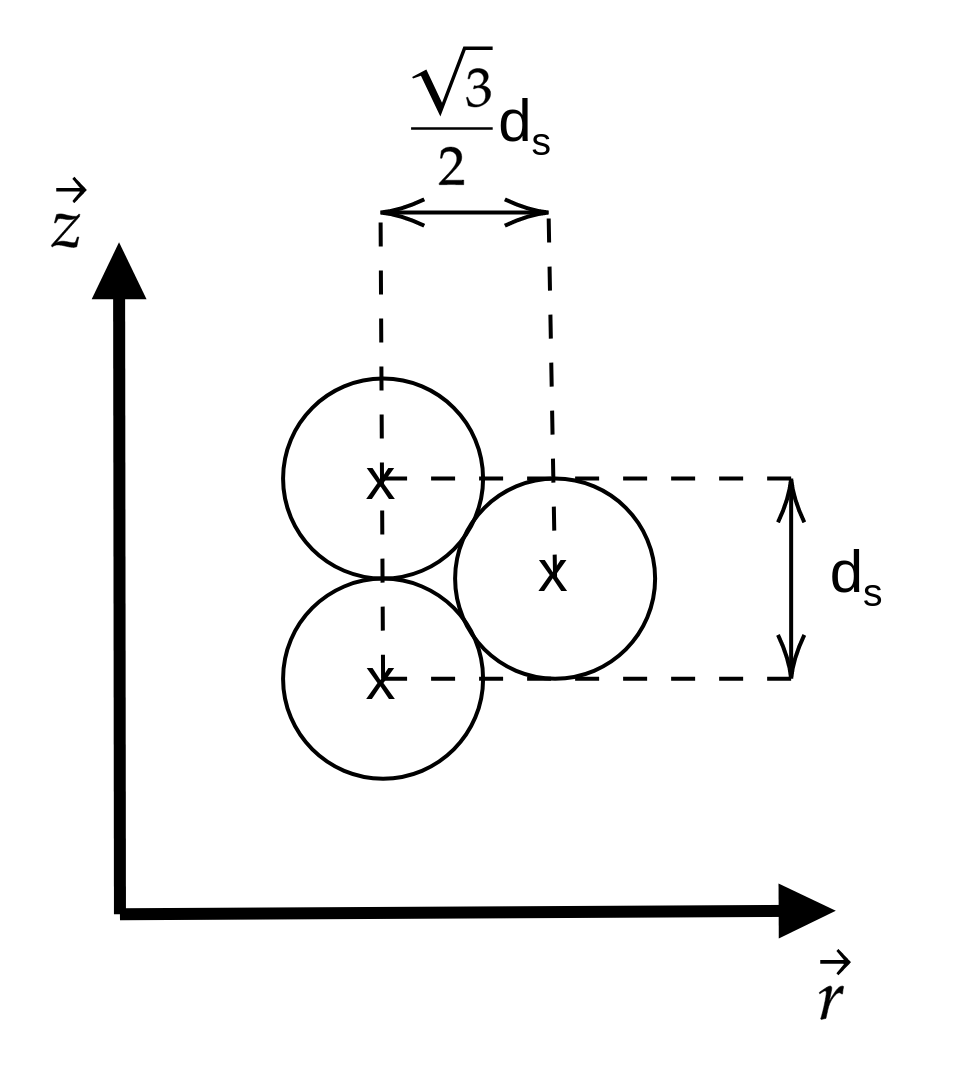
\includegraphics[height=0.3\textwidth]{schema_packing.png}
    \caption{Schematic of the packing of DNA strands.}
    \label{fig:hexagone}
\end{figure}

Putting all these expressions together, we obtain bending energy:
\begin{eqnarray}
    G_{bend} &=& \frac{2 \pi \xi_p k_B T}{\sqrt{3} d_s^2} \int_{R_{int}}^{R_{out}} \frac{h(R)}{R} dR
\end{eqnarray}

We see that the bending term takes into account the rigidity of the polymer and the shape of the capsid. The latter will be encoded in the $h$ function. We come back to the computations for different shapes later, for now let us look at the repulsion term.

\subsubsection{DNA-DNA repulsion}

The other term that must be taken into account in the energy of the system is the repulsion between DNA strands. In fact, each base pair is charged with a charge $+2$ \cite{alberts2002} and DNA is a strongly charged molecule $ \sim 7 C.nm^{-1} $. Due to this charge, DNA could not be stable if it was not in a solution containing counter ions \cite{singh2015}. In this model we will only consider interaction between nearest neighbours. Once again this choice is based on the assumption that the spool is always very well organized.

The force has been determined experimentally based on measurements of osmotic pressure. The force between two unit length DNA strands seperated by a distance $d_s$ is : $g_{el} \left(d_s\right) = \frac{F_0 d_s}{\sqrt{3}} exp \left(\frac{-d_s}{c}\right) $, where $F_0$ is homogeneous to a force per unit length and $c$ to a length. These are parameters that should be determined from fits on experimental data. The form of this expression comes from the fact that the ions in the solution tend to screen the charge of the DNA strands. That is why we do not have a behaviour in $\frac{1}{d_s^2}$ as one might expect for Coulomb repulsion. No direct measurement of $F_0$ and $c$ have been done to our knowledge \cite{purohit2003}. $g_{el}$ represents the potential energy of interaction of two DNA strands of unit length at a distance $d_s$ from one to another. To compute the potential energy of interaction of two unit length of strand we have to compute the energy we bring two strands that are separated by an infinity distance, to $d_s$ between them. By doing so we compute the energy of one link between two DNA strands.

\begin{eqnarray*}
    G_{el}^{link} &=& \int_{\infty}^{d_s} f_{el} \left( d'_s \right) dd'_s \\
    & = & \int_{\infty}^{d_s} \frac{F_0 d'_s}{\sqrt{3}} exp \left(\frac{-d'_s}{c}\right) dd'_s \\
    & = & \frac{F_0}{\sqrt{3}} \left( c^2 + cd_s \right) exp \left( \frac{- d_s}{c} \right) \;\; \textnormal{(we made an intergration by part)} \label{eq:gelec}
\end{eqnarray*}

As each strand has six neighbours and each link is between two strands (see figure \ref{fig:lattice}) we have to put a factor 3. Then we have to multiply this energy by unit length along full length of the DNA strand:
\begin{eqnarray}
    G_{charge} &=& 3 L G_{el}\left(ds\right) = L\sqrt{3} F_0 \left( c^2 + cd_s \right) exp \left( \frac{- d_s}{c} \right) \label{eq:gcharge}
\end{eqnarray}

\begin{figure}[H]
    \centering
    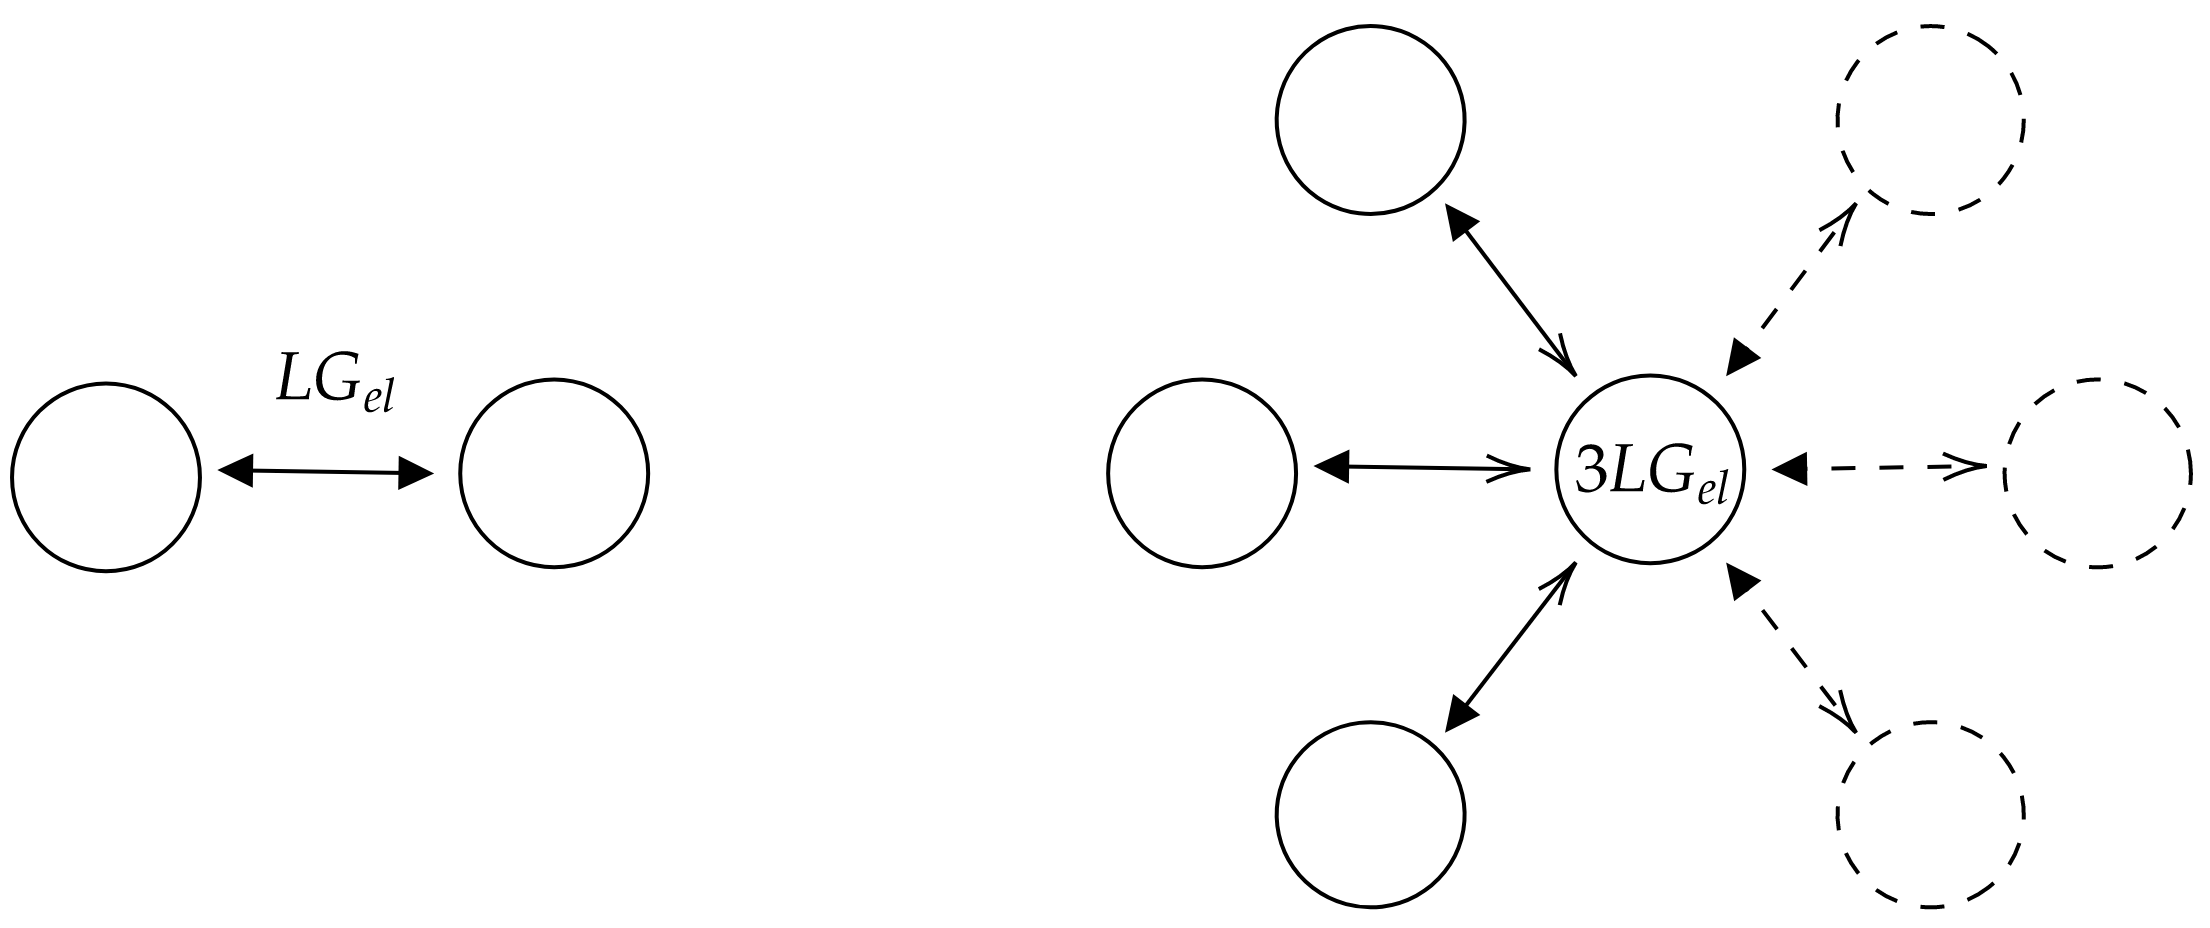
\includegraphics[width=0.5\textwidth]{diagram_Gcharge.png}
    \caption{Repulsion between DNA strand.}
    \label{fig:lattice}
\end{figure}

The expression might seem very simple. In fact it also contain a dependence in the geometry of the capsid. This dependence is hidden in L. The length of DNA in the capsid reads (see the appendix equation \ref{eq:Ldef}):

\begin{eqnarray*}
    L & = & \frac{4 \pi}{\sqrt{3} d_s^2} \int_{R_{int}}^{R_{out}} R h(R) dR
\end{eqnarray*}

We have derived the explicit expression for each term in the hamiltonian. Now what we want to do is put everything together and minimize the hamiltonian. This is done in the next section.

\subsection{The equation on $d_s$}

In this section we are going to minimize analytically the expression of $G$. This approach rely on the fact that at mechanical equilibrium the DNA strands are just lying in the configuration such that the energy is minimised. As the length of DNA inside the capsid is fixed, the only parameter that can be optimised is $d_s$. Let us write the full expression of G:

\begin{eqnarray}
    G_{tot} &=& \frac{2 \pi \xi_p k_B T}{\sqrt{3} d_s^2} \int_{R_{int}}^{R_{out}} dR \frac{h(R)}{R} + L \sqrt{3} F_0 \left( c^2 +cd_s \right) \exp{ \left( \frac{d_s}{c} \right) }
    \label{eq:Gtot}
\end{eqnarray}

Writing the condition $ \frac{d G_{tot}}{d d_s} = 0 $ leads to the equation:
\begin{eqnarray}
    \sqrt{3} F_0 \exp{ \left( \frac{-d_s}{c} \right) } &=& \frac{\xi_p k_B T}{d_s^2 R_{int}^2} - \frac{\xi_p k_B T}{2 d_s^2} \frac{\int_{R_{int}}^{R_{out}} \frac{h(R)}{R} dR}{\int_{R_{int}}^{R_{out}} R h(R) dR} 
    \label{eq:deriv_ds_final}
\end{eqnarray}

We see that this is a closed hierarchy and that it can in principle be solved. Analytical solving does not seem to be at hand. So for this we need to rely on numerical solving of this equation.

\subsection{The force during packing}
Now let us imagine that we have found the value of $d^*_s$ that minimises the free energy. We can reintroduce it in $G$ and deduce the motor force via $F=\frac{d G}{d L}$. We deduce from equation (\ref{eq:Gtot}) that (see appendix \ref{sec:appenForce} for detailed derivation):
\begin{eqnarray}
    F &=& \frac{\xi_p k_B T}{2 R_{int}^2} + F_0 \sqrt{3} \left( c^2 + c d_s^* \right) \exp{ \left( \frac{-d^*_s}{c} \right) }
    \label{eq:F}
\end{eqnarray}

This is exactly the expression that have been given in \cite{purohit2003} (see equation [19] of the reference).
As a conclusion, we have seen how to derive the expression for the force of the motor. Now we want to find a more explicit form for this force. We would like to express the force as a function of the percentage of DNA packed inside the capsid. We will see in the next section that for that we need to specialise to a given geometry of capsid.

\section{Computing of the force in various geometries}

In this section we will show that for typical geometry of capsid, we can express the force as a fucntion of the percentage of DNA packed inside the capsid, the radius $R_{out}$ and the rate of compaction $\rho_{pack} = \frac{\Omega_{dna}}{\Omega_{caps}}$ (it the ratio of the volume occupied by the DNA when it is fully packed divided by the volume of the capsid). We remark here that $ \Omega_{dna} = \frac{\sqrt{3}d_s^2}{2} L$. It is interesting to use these three parameters corresponds to quantity that are easy to access experimentally \cite{phillips2005, purohit2003}. We will dsitinguish three geometry of capsid : (1) \emph{cylindrical}, when the capsid is a cylindre, (2) \emph{spherical}, when the capsid is sphere, (3) \emph{spherical-capped}, when the capsid is a cylinder capped with two hemispheres (see figure \ref{fig:shapes}).

\begin{figure}[H]
    \centering
    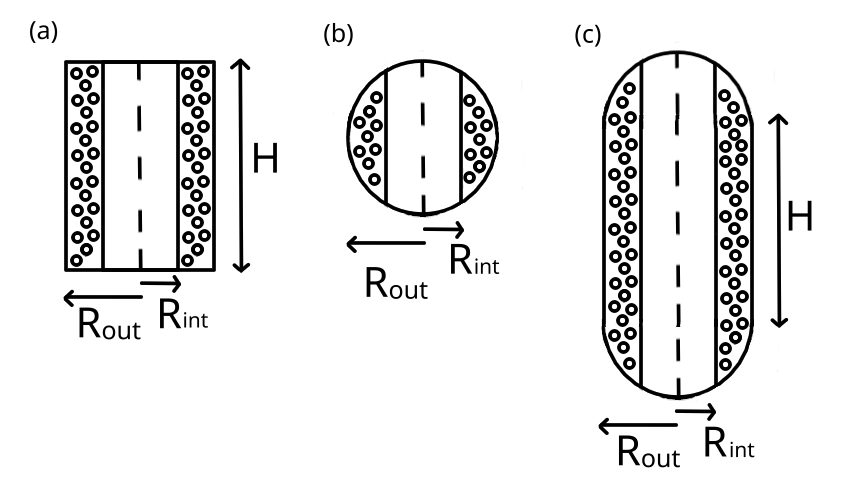
\includegraphics[width=0.7\textwidth]{analitical_geometries.png}
    \caption{Geometries that will be studied analytically: (a) is a simple cylindrical capsid, (b) is a spherical capsid and (c) is a capped cylindrical capsid.}
    \label{fig:shapes}
\end{figure}

To compute the force we will need to express the following quantities (see the equations below) as a function of $d_s$, $\rho_{pack}$, $ p $ which is the percentage of DNA that have been packed. These quantity can be expressed as a function of $R_{int}$ but it hides the dependency in $d_s$. We will repress this quantidy in terms of the variables $d_s$, $\rho_{pack}$, $ p $.

\begin{eqnarray}
    \int_{R_{int}}^{R_{out}} 2 \pi h(R)RdR &=& - \frac{d_s^2 \sqrt{3}}{2}L \\
    \int_{R_{int}}^{R_{out}} dR \frac{h(R)}{R} & & \\
    \rho_{pack} &=& \frac{\Omega_{dna}}{\Omega_{caps}} \\
    A &=& \frac{\xi_p k_B T}{R_{int}^2} - \xi_p k_B T \frac{\int_{R_{int}}^{R_{out}} \frac{h(R)}{R} dR}{\int_{R_{int}}^{R_{out}} R h(R) dR} \\
    & & \text{Which is useful to compute the right hand side of (\ref{eq:deriv_ds_final}}) \\
    G_{bend} & & \\
    G_{charge} & &
\end{eqnarray}

\begin{figure}[H]
    \centering
    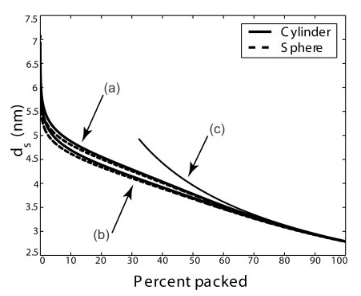
\includegraphics[width=0.5\textwidth,height=0.4\textwidth]{ds_vs_packing_ratio.png}
    \caption{Spacing between DNA strands as a function of the percent of genome packed for cylindrical and spherical capsid geometries. We assume repulsive solvent conditions with $F0~=~255,000~pN/nm^2$ (a) or $F0~=~4.1~\times~55,000~pN/nm^2$ (b). The capsid dimensions are chosen so their volumes coincide with the $\phi~29$ virus. Curve (c) is the spacing between strands assuming a uniform packing of the capsid. Figure and legend taken from: \cite{purohit2003}.}
    \label{fig:enter-label}
\end{figure}

\subsection{Cylindrical capsid}

For the cylindrical capsid, the starting point is $h(R) = h$.
We deduce:
\begin{eqnarray}
    \int_{R_{int}}^{R_{out}} h 2 \pi R dr &=& \frac{d_s^2 \sqrt{3}}{2}L \\
    R_{int} &=& R_{out} \sqrt{1 - \frac{\sqrt{3}d_s^2L}{2 \pi h R_{out}^2}} \\
    \rho_{pack} &=& \frac{d_s^2 \sqrt{3} L}{2} \frac{1}{\pi h R_{out}^2} \\
    \int_{R_{int}}^{R_{out}} dR \frac{h(R)}{R} & = & -\frac{h}{2} \ln \left( 1-\rho_{pack}\right) \\
    A & = &\frac{\xi_p k_B T}{R_{out}^2} \left[ \frac{1}{ \left( 1 - \rho_{pack} p\right)} - \frac{\ln \left( 1-\rho_{pack}p \right) }{\rho_{pack} p} \right] \\
    G_{bend} &=& \frac{2 \pi k_B T h}{\sqrt{3} d_s^2} \ln \left( \frac{R_{out}}{R_{int}} \right) \\
    G_{charge} &=& L \sqrt{3} \left( c^2 + c d_s \right) \exp \left( \frac{-d_s}{c} \right)
\end{eqnarray}

Now to compute the force during the packing, we need to varie p from 0 to 1. For each value of p we compute $d_s$ (\ref{eq:cylds}). We can deduce the expression of the force via (\ref{eq:cylF}).
\begin{equation}
    0 = \sqrt{3} F_0 \exp \left( \frac{-d_s}{c} \right) - \frac{\xi_p k_B T}{R_{out}^2 d_s^2} \left[ \frac{1}{ \left( 1 - \rho_{pack} p\right)} - \frac{\ln \left( 1-\rho_{pack}p \right) }{\rho_{pack} p} \right] 
    \label{eq:cylds}
\end{equation}

\begin{equation}
    F = \frac{2 \pi \xi_p k_B T}{2 R_{out}^2 \left( 1 - \frac{d_s^2 \sqrt{3} L}{2} \frac{1}{\pi h R_{out}^2}\right) } + F_0 \sqrt{3} \left( c^2 + cd_s \right) \exp \left( \frac{-d_s}{c} \right) \\
    \label{eq:cylF}
\end{equation}

We where able to implement these expression numerically and find back at a qualitative level the plot presented in \cite{purohit2003}. Here we have considered that L is the length of the DNA strand (in full) which means that when it is not fully packed, one should replace $L$ by $L\times p$ (this is true in all the above expressions).

\begin{figure}
    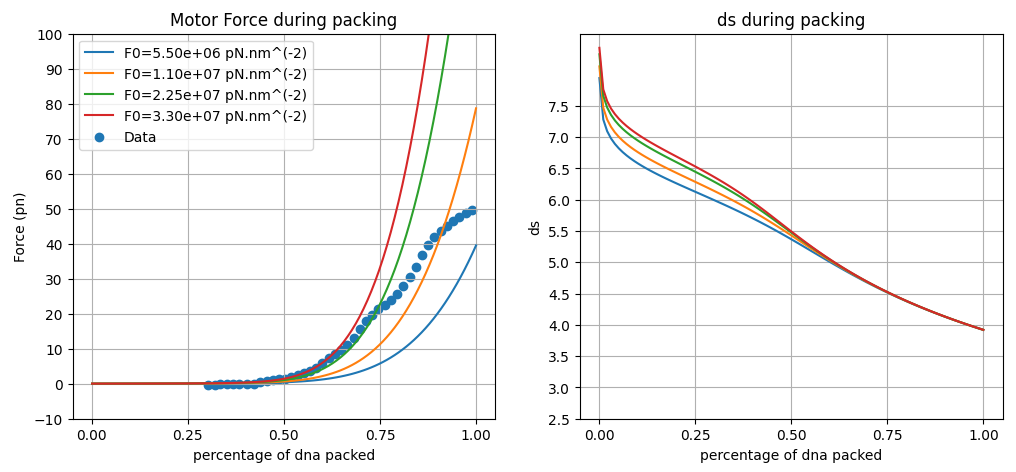
\includegraphics[width=\textwidth]{Plot_ofTheForce_Cyl.png}
    \caption{We implemented these expressions in python. For each step, we set the parameter $p$ (percentage of DNA packed) determine $d_s$ via a the routine \url{scipy.optimize.root()}. We used the \url{'lm'} (Levenberg-Marquart) method (other method where not achieving to converge). Then, usind $d_s$ and $p$ one can compute the force. The parameters we used are : $k_B=1.380.10^{-23}JK^{-1}$, $T=310 K$, $R_{out} = 47 nm$, $h = 37.9 nm$, $ \xi_p = 25 nm$, $L = 3*6.584e3 nm$, $c_0 = 0.27 nm$ (close to \cite{purohit2003})}
\end{figure}

We observe an evolution of $d_s$ that seems pseudo-exponential around $0$. This is because at first the strand will minimise their energy by being packed as far away from each other as possible, but will very quickly pack closer to each other to then be able to have a large enough bend radius; thus moving to the next regime we observe.

We then observe a seemingly linear decrease in $d_s$ with the packing percentage, as decreasing $d_s$ is a trade-off between allowing more strand to have a larger bending radius thus minimising the bending energy, and having strands closer together thus increasing the repulsion energy.

We also observe a slight change of regime in the evolution of $d_s$ between $p \in \left[5\%,\;45\%\right]$ where the trajectory of $d_s$ is affected by $F0$, and $p \in \left[45\%,\;100\%\right]$ where the trajectory of $d_s$ is independent (and smilingly in continuity with the trajectory found at small $F0$).

We can thus suppose that for small packing percentages ($p \in \left[5\%,\;45\%\right]$) the repulsion energy ($G_{charge}$ dependent in $F0$) has a significant impact, whereas for large packing percentages ($p \in \left[45\%,\;100\%\right]$) the bending energy ($G_{bend}$) dominates the determination of $d_s$. This can be qualitatively understood by the fact that for high packing percentages, smaller and smaller bend radius occur.

Finally we observe that our model for the force properly describe the evolution of the experimentally observed packing force for $F0=2.25.10^7pN.nm^{-2}$ for packing percentages $p \leq 75\%$. For packing percentages greater than $75\%$ our model doesn't describe the inflection of the force.

\subsection{Spherical capsid}
We can do the same job for a spherical capsid.
\begin{eqnarray}
    h(R) &=& 2 R_{out} \sqrt{1 - \frac{R^2}{R_{out}^2}}\\
    R_{int} &=& \left(1 - \left( \frac{d_s^2 L \sqrt{3}}{2 \frac{4\pi}{3} R_{out}^3} \right) ^{\frac{2}{3}}\right)^{\frac{1}{2}} R_{out} \\
    \rho_{pack} &=& \frac{\frac{\sqrt{3}}{2} d_s^2 L}{\frac{4}{3} \pi R_{int}^3} \\
    \int_{R_{int}}^{R_{out}} dR \frac{h(R)}{R} & = & -2 R_{out} \left[ \ln \left( \left( 1 - \rho_{pack}^{2/3}\right)^{-1/2} - \frac{\rho_{pack}^{1/3}}{\sqrt{ \left(1 - \rho_{pack}^{2/3}\right)}} \right) + \rho_{pack}^{1/3} \right] \\
    \int_{R_{int}}^{R_{out}} dR h(R) R &=& \frac{2}{3} R_{out}^3 \left( 1 - \frac{R_{int}^2}{R_{out}^2} \right)^{3/2} \\
    A &=& \frac{\xi_{p} k_B T }{R_{out}^2 \left( 1 - \rho_{pack}^{2/3} \right)} - \frac{3 \xi_p k_B T}{2 R_{int}} \left[ \frac{ \ln \left\{ \left(  1 - \rho_{pack}^{2/3} \right)^{-1/2} - \frac{\rho_{pack}^{1/3}}{\sqrt{ \left(1 - \rho_{pack}^{2/3}\right)}} \right\} + \rho_{pack}^{1/3}}{\rho_{pack}} \right] \\
    G_{bend} &=& \frac{-4 \pi \xi_p k_B T R_{out}}{\sqrt{3} d_s^2} \left[ \ln \left\{ \left( 1 - \rho_{pack}^{2/3} \right)^{-1/2} - \rho^{1/3} \left( 1 - \rho_{pack}^{2/3} \right)^{-1/2} \right\} + \rho_{pack}^{1/3} \right] \\
    F &=& \frac{ \xi_p k_B T}{2 R_{out}^2 \left( 1 - \rho_{pack}^{2/3} \right) } + F_0 \sqrt{3} \left( c^2 + c d_s \right) \exp \left( \frac{-ds}{c} \right)
\end{eqnarray}

We weren't able to do the same numerical analysis as for the cylindrical capsid as our numerical solver didn't obtain a stable solution for $d_s$ given the properties of the energy for this capsid geometry.

However looking as the equation we obtained in comparison with the one obtained for the cylindrical capsid, we can mainly observe that the force has a different order in $p_{pack}$ ($-\frac{2}{3}$ for the spherical capsid versus $-1$ for the cylindrical capsid).

This difference can be qualitatively explained by the fact that the bend radius will decrease quicker for the spherical capsid as the vertical section of the capsid for a given radius is decreasing with a decreasing radius.

We could hypothesis given the insights of the numerical analysis for the cylindircal capsid that this would lead to a transition to a regime where $F0$ isn't determinant in the dynamic of $d_s$ for smaller packing radiuses.

\subsection{Capped cylindrical capsid}

We will now do the same analysis as in the previous section, but using a different geometry:

\begin{eqnarray}
    h(R) &=& H + 2Rout \sqrt{1 - \frac{R^2}{R_{out}^2}} \\
    \rho_{pack} &=& \frac{ \frac{4}{3}\pi R_{out}^3 \left( 1 - \frac{R_{int}^2}{R_{out}^2} \right)^{3/2} + \pi H R_{out}^2 \left( 1 - \frac{R_{int}^2}{R_{out}^2} \right) }{ \frac{4}{3} \pi R_{out}^3 + \pi H R_{out}^2 } \\
    G_{bend} & = & \frac{\pi k_B T \xi_p}{3 d_s^2} \left[ H \ln \left( \frac{R_{out}}{R_{int}} \right)  + 2R_{out} \ln \left( \frac{\sqrt{R_{out}^2 - R_{int}^2} + R_{out}}{R_{int}} \right) - 2 R_{out} \sqrt{\left( 1 - \frac{R_{int}^2}{R_{out}^2} \right)} \right] \\
    \frac{\sqrt{3}d_s^2}{2} L & = & \pi H R_{out}^2 \left( 1 - \frac{R_{int}^2}{R_{out}^2} \right) + \frac{4\pi}{3} R_{out}^3 \left( 1 - \frac{R_{int}^2}{R_{out}^2} \right)^\frac{3}{2} \\
    A &=& \frac{\xi_p k_B T}{R_{int}^2} + \frac{\xi_p k_B T}{2} \frac{ H \ln \left\{ \left( \frac{R_{out}}{R_{int}} - R_{out}\right) - \sqrt{ 1 - \frac{R_{int}^2}{R_{out}^2}} \right\} - \ln \left\{ \frac{R_{out}}{R_{int}} \right\} - \sqrt{\frac{R_{out}^2}{R_{int}^2}-1}}{\frac{4\pi}{3} R_{out}^3 \left( 1 - \frac{R_{int}^2}{R_{out}^2}\right)^{3/2} + \pi H R_{out}^2 \left( 1 - \frac{R_{int}^2}{R_{out}^2} \right) }
\end{eqnarray}

This very last expression could in principle be used to express $R_{int}$ it is doable analytically with help of a formal calculus program like Wolfram. But the expression obtained are so cumbersome that we will not even try to present them here. Expressing everything in terms of $\rho_{pack}$ seems hopeless.

In the impossibility of doing a numerical analysis, we can qualitatively say that the capped cylindrical capsid has two limits: for $R_{out} \gg H$ we end up with a capsid that can be considered spherical. In the opposite limit, for $H \gg R_{out}$ we end up with a capsid that will be dominated by its thin cylindrical body, and can thus be analysed in this limit.

\section{Conclusion}

We were able through a physical description of the DNA packing dynamic, and through analytical computation to describe the different terms contribution to the energy taken to pack DNA.

We were then capable of using theses computation to numerically obtain results for the simpler cylindrical capsid geometry, and get a qualitative understanding of these results which we could carry over to the other capsid geometry which we were not able to numerically analyse.

We were also able to separate the packing process between two regime were different contribution would decide the inter-strand spacing. We were however unable to explain the inflection observed in the real packing force as our model's packing force has a continuous exponential growth in the force with the packing percentage.

% \subsection{Capsid geometry comparison} \label{sec:quali}


% \section{Computing of the force in various geometries}

% In this section we will show that for typical geometry of capsid, we can express the force as a fucntion of the percentage of DNA packed inside the capsid, the radius $R_{out}$ and the rate of compaction $\rho_{pack} = \frac{\Omega_{dna}}{\Omega_{caps}}$ (it the ratio of the volume occupied by the DNA when it is fully packed divided by the volume of the capsid). We remark here that $ \Omega_{dna} = \frac{\sqrt{3}d_s^2}{2} L$. It is interesting to use these three parameters corresponds to quantity that are easy to access experimentally \cite{phillips2005, purohit2003}. We will dsitinguish three geometry of capsid : (1) \emph{cylindrical}, when the capsid is a cylindre, (2) \emph{spherical}, when the capsid is sphere, (3) \emph{spherical-capped}, when the capsid is a cylinder capped with two hemispheres (see figure \ref{fig:shapes}).

% \begin{figure}[H]
%     \centering
%     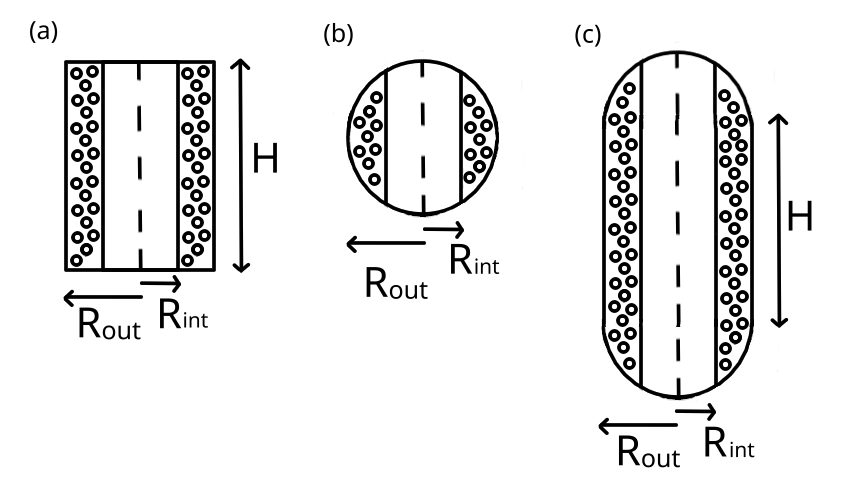
\includegraphics[width=0.7\textwidth]{analitical_geometries.png}
%     \caption{Geometries that will be studied analytically: (a) is a simple cylindrical capsid, (b) is a spherical capsid and (c) is a capped cylindrical capsid.}
%     \label{fig:shapes}
% \end{figure}

% To compute the force we will need to express the following quantities (see the equations below) as a function of $d_s$, $\rho_{pack}$, $ p $ which is the percentage of DNA that have been packed. These quantity can be expressed as a function of $R_{int}$ but it hides the dependency in $d_s$. We will repress this quantidy in terms of the variables $d_s$, $\rho_{pack}$, $ p $.

% \begin{eqnarray}
%     \int_{R_{int}}^{R_{out}} 2 \pi h(R)RdR &=& - \frac{d_s^2 \sqrt{3}}{2}L \\
%     \int_{R_{int}}^{R_{out}} dR \frac{h(R)}{R} & & \\
%     \rho_{pack} &=& \frac{\Omega_{dna}}{\Omega_{caps}} \\
%     A &=& \frac{\xi_p k_B T}{R_{int}^2} - \xi_p k_B T \frac{\int_{R_{int}}^{R_{out}} \frac{h(R)}{R} dR}{\int_{R_{int}}^{R_{out}} R h(R) dR} \\
%     & & \text{Which is useful to compute the right hand side of (\ref{eq:deriv_ds_final}}) \\
%     G_{bend} & & \\
%     G_{charge} & &
% \end{eqnarray}

% \begin{figure}[H]
%     \centering
%     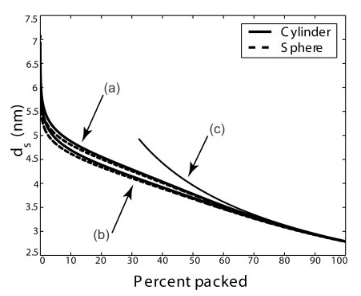
\includegraphics[width=0.5\textwidth,height=0.4\textwidth]{ds_vs_packing_ratio.png}
%     \caption{Spacing between DNA strands as a function of the percent of genome packed for cylindrical and spherical capsid geometries. We assume repulsive solvent conditions with $F0~=~255,000~pN/nm^2$ (a) or $F0~=~4.1~\times~55,000~pN/nm^2$ (b). The capsid dimensions are chosen so their volumes coincide with the $\phi~29$ virus. Curve (c) is the spacing between strands assuming a uniform packing of the capsid. Figure and legend taken from: \cite{purohit2003}.}
%     \label{fig:interstrand_space}
% \end{figure}

% \subsection{Cylindrical capsid}


% For the cylindrical capsid, we have $h(r) = H$. We thus have the bending energy $G_{bend}$:

% \begin{eqnarray}
%     %G_{bend} & = & \int_{R}^{R_{out}} \frac{k_B T \xi_p}{2\sqrt{3}} N(r)  \left( \int_{0}^{2\pi r} \frac{1}{r^2} dl \right) \frac{dr}{d_s} =  \frac{\pi k_B T \xi_p}{\sqrt{3}d_s^2} \int_{R}^{R_{out}} \frac{h(r)}{r} dr \\
%     G_{bend}^{cylinder} & = & \frac{2\pi \xi_p k_B T}{\sqrt{3}d_s^2} ln \left( \frac{R_{out}}{R_{int}} \right) H 
% \end{eqnarray}

% And also the electronic repulsion energy $G_{charge}$, assuming that we have hexagonal packed parallel strands of length $2\pi r$:

% \begin{eqnarray}
%     L^{cylinder} & = & \frac{2 \pi }{\sqrt{3}d_s} \left( R_{out}^2 - R_{int}^2 \right) H \\
%     G_{charge}^{cylinder} & = & 3 G_{el}(d_s) L^{cylinder} = \frac{2 \sqrt{3} \pi G_{el}(d_s)}{d_s} \left( R_{out}^2 - R_{int}^2 \right) H
% \end{eqnarray}

% %Identifying the inserted length $L$:
% %\begin{eqnarray}
% %    %L & = & \frac{2 \pi}{\sqrt{3}d_s} \int_{R}^{R_{out}} r h(r) dr \\
% %    L^{cylinder} & = & \frac{2 \pi }{\sqrt{3}d_s} \left( R_{out}^2 - R_{int}^2 \right) H
% %\end{eqnarray}

% We can then compute the force by derivating relativly to the inserted length:

% \begin{eqnarray}
%     F_{mot} & = & -\frac{\partial G_{tot}}{\partial L} \\
%     F_{mot}^{cylinder} & = & -3 G_{el}(d_s) + \frac{\xi_pk_B T}{2R_{int}^2} = -\sqrt{3}F_0(c^2 + cd_s)\exp(-\frac{d_s}{c}) + \frac{\xi_pk_BT}{2(R_{out}^2 - \frac{\sqrt{3}d_s^2L}{2\pi H})}
% \end{eqnarray}

% \subsubsection{Minimizing the energy}

% Assuming that in the stationary state, the capsid it at the mechanical equilibrium, the value of $d_s$ is the one that minimises the total energy. We minimise: $G_{tot}(d_s) = G_{bend} + G_{charge}$:

% \begin{eqnarray}
%     \frac{\partial G_{tot}}{\partial d_s} & = & 0 = - \frac{2 \pi k_B T \xi_p}{\sqrt{3}d_s^3}  ln \left( \frac{R_{out}}{R_{int}} \right) H + \pi F_0 \left[  1 - 3 \frac{ c  }{d_s} - 3\frac{ c^2 }{d_s^2} \right] exp \left(\frac{-d_s}{c}\right) \left( R_{out}^2 - R_{int}^2 \right) H
% \end{eqnarray}

% This equation is not generally solvable for any $L$, they are thus solved numerically \cite{purohit2003}.

% However we see that the $d_s$ has a known evolution which we can assume as true to give us a qualitative understanding of the evolution of the force and of the other various properties.

% \subsection{Spherical capsid}

% For the spherical capsid, the number of packaged hoops at radius R is $N(R) = \frac{h(R)}{ds}$, with $h(R) = 2\sqrt{R_{out}^2 - R^2}$ being the length of the column of hoops. The bending and interaction contributions are thus:

% \begin{eqnarray}
%     G^{sphere}_{bend} &=& \frac{-4\pi\xi_pk_BT}{\sqrt{3}d_s^2}\bigg[\sqrt{R_{out}^2 - R_{int}^2} + R_{out}\ln\bigg(\frac{R_{out} - \sqrt{R_{out}^2 - R_{int}^2}}{R_{int}}\bigg)\bigg] \\
%     G^{sphere}_{charge}  &=& \frac{8\pi}{3d_s^2}F_0(c^2 + cd_s) (R_{out}^2 - R_{int}^2)^\frac{3}{2}\exp(-\frac{d_s}{c})
% \end{eqnarray}

% Differentiating each term in the free energy with regards to the packaged length $L(R_{int}) =  \frac{8\pi}{3\sqrt{3}d_s^2}(R_{out}^2 - R_{int}^2)^\frac{3}{2}$, we obtain the following total force:
% \begin{eqnarray}
% F_{tot}^{sphere} = -\sqrt{3}F_0(c^2 + cd_s)\exp(-\frac{d_s}{c}) +  \frac{\xi_pk_BT}{2(R_{out}^2 - (\frac{3\sqrt{3}d_s^2L}{8\pi})^\frac23)}    
% \end{eqnarray}

% where we assumed that $d_s$ is constant and given by the minimizing condition for the total free energy:

% \begin{eqnarray}
%     \sqrt{3}F_0\exp(-\frac{d_s}{c}) = \frac{\xi_pk_BT}{R_{int}^2d_s^2} + \frac{3\xi_pk_BT}{d_s^2}\bigg[\frac{1}{R_{out}^2 - R_{int}^2} + \frac{R_{out}}{^(R_{out}^2 - R_{int}^2)^\frac32}ln\bigg(\frac{R_{out} - \sqrt{R_{out}^2 - R_{int}^2}}{R_{int}}\bigg) \bigg] 
% \end{eqnarray}

% As for the previous geometry, we can rewrite the expression for the force in terms of the packing density $\rho_{pack}  = \frac{\frac{\sqrt{3}}{2}d_s^2L}{\frac43 \pi R_{out}^3}= \frac{3\sqrt{3}d_s^2L}{8\pi  R_{out}^3}$:

% \begin{eqnarray}
% F_{tot}^{sphere} = -\sqrt{3}F_0(c^2 + cd_s)\exp(-\frac{d_s}{c}) +  \frac{\xi_pk_BT}{2R_{out}^2(1 - \rho_{pack}^\frac23)}    
% \end{eqnarray}

% \subsection{Capped cylindrical capsid}

% We will now do the same analysis as in the previous section, but using a different geometry:

% \begin{eqnarray}
%     G_{bend}^{capped\_cyl.} & = & \frac{\pi k_B T \xi_p}{3 d_s^2} \int_{R_{int}}^{R_{out}} \frac{h + 2 R \sqrt{1 - \frac{r^2}{R_{out}^2}}}{r} dr \\
%     & = & \frac{\pi k_B T \xi_p}{3 d_s^2} \left[ h \ln \left( \frac{R_{out}}{R_{int}} \right)  + 2R_{out} \ln \left( \frac{\sqrt{R_{out}^2 - R_{int}^2} + R_{out}}{R_{int}} \right) - 2 R_{out} \sqrt{\left( 1 - \frac{R_{int}^2}{R_{out}^2} \right)} \right] \\
%     L^{capped\_cyl.} & = & \frac{\pi }{\sqrt{3}d_s} \left( R_{out}^2 - R_{int}^2 \right) H + \frac{8\pi}{3\sqrt{3}d_s^2}(R_{out}^2 - R^2)^\frac{3}{2} \\
% \end{eqnarray}
% To obtain $G_{charge}$ we can simply remark that it is the sum of the $G_{el}$ in the spherical capsid and the one in the cylindrical capsid. We obtain:
% \begin{eqnarray}    
%     G_{charge}^{capped\_cyl.} & = & \frac{\sqrt{3} \pi G_{el}(d_s)}{d_s} \left[ \left( R_{out}^2 - R_{int}^2 \right) + \frac{2R_{out}}{3} \left( 1 - \frac{R_{int}^2}{R_{out}^2} \right)^{\frac{3}{2}} \right]
% \end{eqnarray}


% We eliminate the variable $d_s$ in the above equations by minimizing $G_{tot}(d_s) = G_{bend} + G_{charge}$:

% \begin{eqnarray}
%     TODO
% \end{eqnarray}

% \subsection{Capsid geometry comparison} \label{sec:quali}

% \begin{table}[H]
%     \centering
%     \begin{tabular}{|| p{0.1\linewidth} | p{0.25\linewidth} | p{0.3\linewidth}| p{0.3\linewidth} ||}
%         \hline \hline
%         \textbf{Type of geometry} & \textbf{cylindrical capsid (a)} & \textbf{spherical capsid (b)} & \textbf{capped cylindrical capsid (c)} \\
%         \hline \hline
%         $h(R)$ & $H$ & $2\sqrt{R_{out}^2 - R_{int}^2}$ & $H + 2\sqrt{R_{out}^2 - R_{int}^2}$ \\ \hline
%         $L$ & $\frac{2\pi }{\sqrt{3}d_s} \left( R_{out}^2 - R_{int}^2 \right) H$ 
%         & $\frac{8\pi}{3\sqrt{3}d_s^2}\left(R_{out}^2 - R_{int}^2\right)^\frac{3}{2}$ 
%         & $\frac{2\pi }{\sqrt{3}d_s} \left( R_{out}^2 - R_{int}^2 \right) H + \frac{8\pi}{3\sqrt{3}d_s^2}\left(R_{out}^2 - R_{int}^2\right)^\frac{3}{2}$ \\ 
%         \hline
%         $G_{bend}$ & $\frac{2\pi \xi_p k_B T}{\sqrt{3}d_s^2} ln \left( \frac{R_{out}}{R_{int}} \right) H$ 
%         & $\frac{-4\pi\xi_pk_BT}{\sqrt{3}d_s^2}[\sqrt{R_{out}^2 - R_{int}^2} + R_{out}\ln(\frac{R_{out} - \sqrt{R_{out}^2 - R_{int}^2}}{R_{int}})]$ 
%         & TODO \\ \hline
%         $G_{charge}$ & $\frac{6\pi G_{el}(d_s)}{d_s} \left( R_{out}^2 - R_{int}^2 \right) H$ 
%         & $\frac{8\pi}{3d_s^2}F_0(c^2 + cd_s) (R_{out}^2 - R_{int}^2)^\frac{3}{2}\exp(-\frac{d_s}{c})$ 
%         & TODO  \\ \hline
%         $F_{mot}$ & $-\sqrt{3} F_0 \left( c^2 + cd_s \right) exp \left( \frac{- d_s}{c} \right) +  \frac{\xi_pk_B T}{2R_{int}^2}$ & $-\sqrt{3}F_0(c^2 + cd_s)\exp(-\frac{d_s}{c}) +  \frac{\xi_pk_BT}{2(R_{out}^2 - (\frac{3\sqrt{3}d_s^2L}{8\pi})^\frac23)}$ & TODO \\
%         \hline \hline
%     \end{tabular}
%     \caption{Analytical analysis of the various capsid geometries.}
% \end{table}

\clearpage
\FloatBarrier
\printbibliography[
    heading=bibintoc,
    title={References}]

\clearpage
\FloatBarrier

\section*{Appendix}

\subsection*{Details of the computations of section 2}

Length of DNA in the capsid.
\begin{eqnarray}
    L & = & \int_{0}^{L} ds \\
    &=& \int_{R_{int}} ^{R_{out}} 2 \pi R \frac{2 N(R)}{\sqrt{3} d_s} dR \\
    &=& \frac{4 \pi}{\sqrt{3} d_s^2} \int_{R_{int}}^{R_{out}} R h(R) dR
    \label{eq:Ldef}
\end{eqnarray}


\subsection*{Minimization of $G$ \label{sec:Gmin}}

The conformation that DNA will take at steady state is the one corresponding to $d_s$ minimal. We thus have to minimize $G_{tot}$. Let us recall the expression :

\begin{eqnarray*}
    G_{tot} &=& \frac{2\pi \xi_p k_B T}{\sqrt{3} d_s^2} \int_{R_{int}}^{R_{out}} \frac{h(R)}{R} dR + L\sqrt{3} F_0 \left(c^2+cd_s \right) \exp{\left(\frac{-d_s}{c}\right)}
\end{eqnarray*}

We have to take the total derivative of this expression, in $d_s$ when $L$ is constant.
The part on the right of the plus sign, containing the electric repulsion between the strands leads to:
\begin{eqnarray}
    \frac{d G_{charge}}{d d_s} &=& - L \sqrt{3} F_0 d_s \exp{\left(\frac{-d_s}{c}\right)}
    \label{eq:deriv_gcharge}
\end{eqnarray}
Then we have to compute the derivative of the left side of the "$+$" sign. We have to take care that we must not derivate the L but we have to take the derivativ of the integral term which depends implicitly on $d_s$ via $R_{int}$.

Let us first derive some intermediary relation that will show up to be very usefull afterwards.
First let us express the volume of DNA inside the capsid.
\begin{eqnarray}
    \int_{R_{int}}^{R_{out}} 2 \pi R h\left( R \right) dR  &=& \frac{d_s^2 \sqrt{3}}{2} L
    \label{eq:L}
\end{eqnarray}
\begin{eqnarray*}
    \frac{d}{d R_{int}} \int_{R_{int}}^{R_{out}} 2 \pi R h\left( R \right) dR &=& - 2 \pi R_{int} h \left( R_{int} \right) \\
\end{eqnarray*}
\begin{eqnarray}
    \frac{d}{d R_{int}} \int_{R_{int}}^{R_{out}} R h\left( R \right) dR &=& \frac{d_s \sqrt{3} L}{2 \pi} \frac{d d_s}{d R_{int}}
    \label{eq:deriv_1}
\end{eqnarray}

 We use equation (\ref{eq:deriv_1}) to express:
 \begin{equation}
     \frac{d R_{int}}{d d_s} = \frac{-d_s \sqrt{3} L}{2 \pi R_{int} h \left( R_{int} \right)}
     \label{eq:derivativ_rint}
 \end{equation}
We deduce from equations (\ref{eq:derivativ_rint}) that:
\begin{eqnarray}
    \frac{d}{d d_s} \int_{R_{int}}^{R_{out}} dR \frac{h(R)}{R} &=&  \frac{\sqrt{3}L}{2\pi R_{int}^2}
\end{eqnarray}
We can reintroduce this expression in $ G_{bend} $ we have:
\begin{eqnarray}
    \frac{d G}{d d_s} &=& \frac{-2\pi \xi_p k_B T}{\sqrt{3} d_s^3} \int_{R_{int}}^{R_{out}} dR \frac{h(R)}{R} + \frac{k_B T L}{\sqrt{3} R_{int}^2}
    \label{eq:deriv_gbend}
\end{eqnarray}

We can put equations (\ref{eq:deriv_gcharge}, \ref{eq:deriv_gbend}). 
\begin{eqnarray*}
    \frac{d G_{tot}}{d d_s} &=& \frac{\xi_p k_B T}{d_s R_{int}^2} L - \frac{2 \pi \xi_p k_B T}{\sqrt{3} d_s^3} \int_{R_{int}}^{R_{out}} dR \frac{h(R)}{R} - L \sqrt{3} F_0 d_s \exp{ \left( \frac{-d_s}{c} \right)}
\end{eqnarray*}

\begin{eqnarray}
    \sqrt{3}F_0 \exp{ \left( \frac{-d_s}{c} \right)} &=& \frac{\xi_p k_B T}{d_s^2 R_{int}^2 } - \frac{2 \pi \xi_p k_B T}{\sqrt{3} d_s^4} \frac{\int_{R_{int}}^{R_{out}} dR \frac{h(R)}{R}}{L} 
    \label{eq:deriv_ds}
\end{eqnarray}

Using the expression of equation (\ref{eq:L}) we have the expression:
\begin{eqnarray}
    \sqrt{3} F_0 \exp{ \left( \frac{-d_s}{c} \right) } &=& \frac{\xi_p k_B T}{d_s^2 R_{int}^2} - \frac{\xi_p k_B T}{d_s^2} \frac{\int_{R_{int}}^{R_{out}} \frac{h(R)}{R} dR}{\int_{R_{int}}^{R_{out}} R h(R) dR} 
\end{eqnarray}

\subsection*{Computation of the force \label{sec:appenForce}}

In this appendix we drive the expression (\ref{eq:F}). We compute the derivativ of G in L assuming $d_s$ constant. This assumption is valid, because the variation $d d_s$ associated to $dL$ is of higher order. This is not trivial to prove that but it is a reasonable assumption given the shape of the equation of $d_s$ (\ref{eq:deriv_ds_final}).

\begin{eqnarray}
    \frac{d G_{tot}}{d L} &=& \frac{2 \pi k_B T \xi_p}{\sqrt{3} d_s^2} \left( - \frac{h(R_{int})}{R_{int}} \right) \frac{d R_{int}}{d L} + F_0 \sqrt{3} \left( c^2 + c d_s \right) \exp{ \left( \frac{-d_s}{c} \right) }
    \label{eq:F_appendix}
\end{eqnarray}

To compute $\frac{d R_{int}}{d L} $ do as in equation (\ref{eq:L}, \ref{eq:derivativ_rint}) but this time we derive by $L$ keeping $d_s$ constant.
\begin{eqnarray*}
    -R_{int} h(R_{int}) &=& \frac{d_s^2 \sqrt{3}}{4 \pi} \frac{ d L}{d R_{int}} \\
    \frac{d R_{int}}{dL} &=& \frac{ - d_s^2 \sqrt{3} }{ 4 \pi R_{int} h(R_{int}) }
\end{eqnarray*}
Reintroducing this result in (\ref{eq:F_appendix}) we obtain (\ref{eq:F}).

\subsection*{Computation of the force for different geometries}


\subsubsection*{Cylindric capsid}

1. Derivation of the force:

\begin{eqnarray*}
    F_{mot} & = & -\frac{\partial G_{tot}}{\partial L} = -(\frac{\partial G_{charge}}{\partial L} + \frac{\partial R_{int}}{\partial L} \frac{\partial G_{bend}}{\partial R_{int}}) \\
    F_{mot} & = & -3 G_{el}(d_s) - \left( \frac{\partial L}{\partial R_{int}} \right)^{-1} \frac{\partial G_{bend}}{\partial R_{int}} \\
    \frac{\partial L^{cylinder}}{\partial R_{int}} & = & -\frac{4 \pi }{\sqrt{3}d_s^2} H R_{int} \\
    \frac{\partial G_{bend}^{cylinder}}{\partial R_{int}} & = & - \frac{2\pi \xi_p k_B T}{\sqrt{3}d_s^2} \frac{H}{R_{int}}  \\
F_{mot}^{cylinder} & = & -3 G_{el}(d_s) +  \frac{\xi_pk_B T}{2R_{int}^2} = -\sqrt{3}F_0(c^2 + cd_s)\exp(-\frac{d_s}{c}) + \frac{\xi_pk_BT}{2(R_{out}^2 - \frac{\sqrt{3}d_s^2L}{2\pi H})}
\end{eqnarray*}

2. Derivation of the optimal inter-strand spacing:

Using the general equation (\ref{eq:L}), we obtain the following condition for $d_s$:
\begin{eqnarray*}
\sqrt{3}F_0 \exp{ \left( \frac{-d_s}{c} \right)} &=& \frac{\xi_p k_B T}{d_s^2 R_{int}^2 } - \frac{2 G_{bend}^{cylinder}}{Ld_s^2} \\
\sqrt{3}F_0 \exp{ \left( \frac{-d_s}{c} \right)} &=& \frac{\xi_p k_B T}{d_s^2 R_{int}^2 } - \frac{2\xi_p k_B T}{d_s^2}\frac{\ln(\frac{R_{out}}{R_{int}})}{R_{out}^2 - R_{int}^2}
\end{eqnarray*}

\subsubsection*{Spherical capsid}
1. Derivation of the force:
\begin{eqnarray*}
 \frac{\partial G_{charge}^{sphere}}{\partial L} & = &  \sqrt{3}F_0(c^2 + cd_s)\exp(-\frac{d_s}{c}) \\
 \frac{\partial G_{bend}^{sphere}}{\partial L} & = & \left( \frac{\partial L}{\partial R_{int}} \right)^{-1} \frac{\partial G_{bend}^{sphere}}{\partial R_{int}} \\
 \left( \frac{\partial L}{\partial R_{int}}\right)^{-1}  & = & \frac{\sqrt{3}d_s^2}{8\pi R_{int}}\frac{1}{\sqrt{R_{out}^2 - R_{int}^2}} \\
 \frac{\partial G_{bend}^{sphere}}{\partial R_{int}} & = & \frac{4\pi\xi_pk_BT}{\sqrt{3}d_s}[\frac{R_{int}}{\sqrt{R_{out}^2 - R_{int}^2}} - \frac{R_{out}^2}{R_{int}\sqrt{R_{out}^2 - R_{int}^2}}] = \frac{4\pi\xi_pk_BT}{\sqrt{3}d_s} \frac{R_{out}^2 - R_{int}^2}{R_{int}\sqrt{R_{out}^2 - R_{int}^2}}  \\
 \Rightarrow  \frac{\partial G_{bend}^{sphere}}{\partial L} & = & -\frac{\xi_pk_BT}{2R_{int}^2} =-\frac{\xi_pk_BT}{2(R_{out}^2 - (\frac{3\sqrt{3}d_s^2L}{8\pi})^\frac23)}
\end{eqnarray*}
where we used the equation relating the internal radius $R_{int} = \sqrt{R_{out}^2 - (\frac{3\sqrt{3}d_s^2L}{8\pi})^\frac23}$ to the packaged length $L$.

The total force is thus:
\begin{eqnarray*}
    F_{tot}^{sphere} = - \frac{\partial G_{tot}^{sphere}}{\partial L}= -\sqrt{3}F_0(c^2 + cd_s)\exp(-\frac{d_s}{c}) + \frac{\xi_pk_BT}{2(R_{out}^2 - (\frac{3\sqrt{3}d_s^2L}{8\pi})^\frac23)}
\end{eqnarray*}

2. Derivation of the optimal inter-strand spacing:

Using the general equation (\ref{eq:deriv_ds_final}), we obtain the following condition for $d_s$:
\begin{eqnarray*}
\sqrt{3}F_0 \exp{ \left( \frac{-d_s}{c} \right)} &=& \frac{\xi_p k_B T}{d_s^2 R_{int}^2 } - \frac{2 G_{bend}^{sphere}}{Ld_s^2} \\
\sqrt{3}F_0 \exp{ \left( \frac{-d_s}{c} \right)} &=& \frac{\xi_p k_B T}{d_s^2 R_{int}^2 } - \frac{3\xi_p k_B T}{d_s^2}\bigg[\frac{1}{R_{out}^2 - R_{int}^2} + \frac{R_{out}}{^(R_{out}^2 - R_{int}^2)^\frac32}ln\bigg(\frac{R_{out} - \sqrt{R_{out}^2 - R_{int}^2}}{R_{int}}\bigg) \bigg]  
\end{eqnarray*}

\subsubsection*{Capped cylindrical capsid}
For a capped cylinder, our starting point is the height of the capsid as a function of R. 
\begin{eqnarray}
    h(R) &=& h + 2 R_{out} \sqrt{1 - \frac{R_{int}}{R_{out}}} \\
    \frac{\sqrt{3} d_s^2 L}{2} &=& \left[ \frac{4\pi}{3} R_{out}^3 \left( 1 - \frac{R_{int}^2}{R_{out}^2} \right)^\frac{3}{2} + h R_{out}^2 \pi \left( 1 - \frac{R_{int}^2}{R_{out}^2} \right) \right] \\
    
\end{eqnarray}

\end{document}
